\chapter{Simulation der CVD-Precursormoleküle \texorpdfstring{\ce{SiH4}}{Silan} und \texorpdfstring{\ce{O2}}{Sauerstoff}}
\label{appendix_silica}

ReaxFF-Potentiale versprechen die Simulation von Molekülen und deren Reaktion miteinander, die mit den folgenden Simulationen für Silan und molekularen Sauerstoff überprüft werden sollen.
Das endgültige Ziel ist die vollständige Simulation reaktiver Gasphasenabscheidungen mit molekulardynamischen Methoden.

\section{Stabilität der Precursormoleküle}

Simulationen einzelner und mehrerer Precursormoleküle (\ce{SiH4} und \ce{O2}) hinsichtlich ihrer Stabilität wurden im mikrokanonischen sowie im kanonischen Ensemble bei verschiedenen Temperaturen durchgeführt.
Abbildung~\ref{fig:silanestability} zeigt eine Auswahl der Ergebnisse der Silan-Simulationen, an denen sich erkennen lässt, wie instabile Simulationen zur Ablösung der Wasserstoffatome vom Silanmolekül führen.
Bei den Sauerstoff-Atomen wurden keine Auffälligkeiten gefunden.

Die Moleküle wurden mit Materials Studio\cite{biovia_materials_2014} präpariert und anschließend mit einer anfänglichen Temperatur von \SIrange{300}{700}{\kelvin} relaxiert, wobei auf Strukturdaten aus der Literatur zurück gegriffen wurde\cite{haynes_crc_2011}.
Eine Übersicht über die Strukturdaten der in dieser Arbeit dargestellten Moleküle findet sich in Anhang~\ref{appendix_constants}.
%% Eine Strukturoptimierung wurde nicht durchgeführt, da die thermische Stabilität mit Blick auf die künftige Simulation von Reaktionen untersucht werden sollte, für die Energieminimierungen der instabilen Moleküle keinen Mehrwert bringen.
Bei \pot{Al\_Al0\_AlN}, \pot{kulkarni}, \pot{nielson} und \pot{zhang} behalten die Silan-Moleküle ihre Struktur, während bei den anderen Parametrisierungen einige der \ce{Si-H}-Bindungen temperaturunabhängig brechen und so einzelne Wasserstoff-Atome freigeben (Abbildung~\ref{fig:silanestability}).

\begin{figure}[b!h]

  \captionsetup[subfigure]{singlelinecheck=false}
  \def\subfigwidth{0.32\textwidth}
  \begin{subfigure}[t]{3.5cm}
    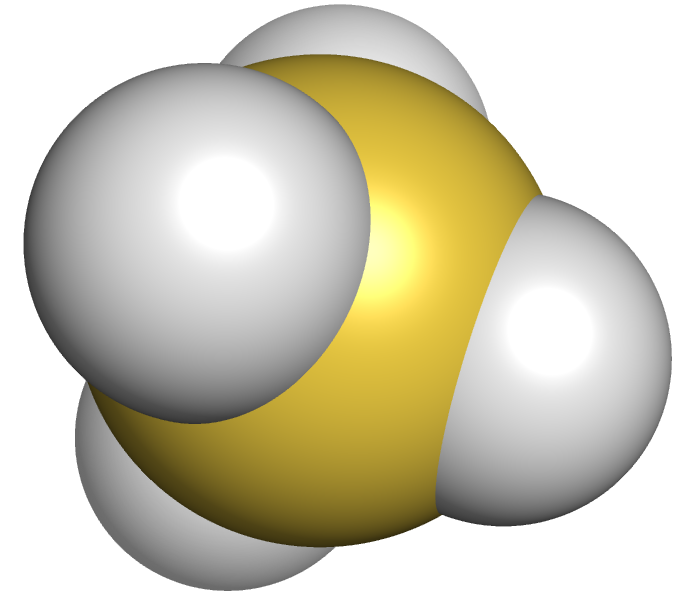
\includegraphics[width=\textwidth]{silane_nielson_stable}
    \subcaption{nielson: stabil}
  \end{subfigure}
  \hfill
  \begin{subfigure}[t]{4.5cm}
    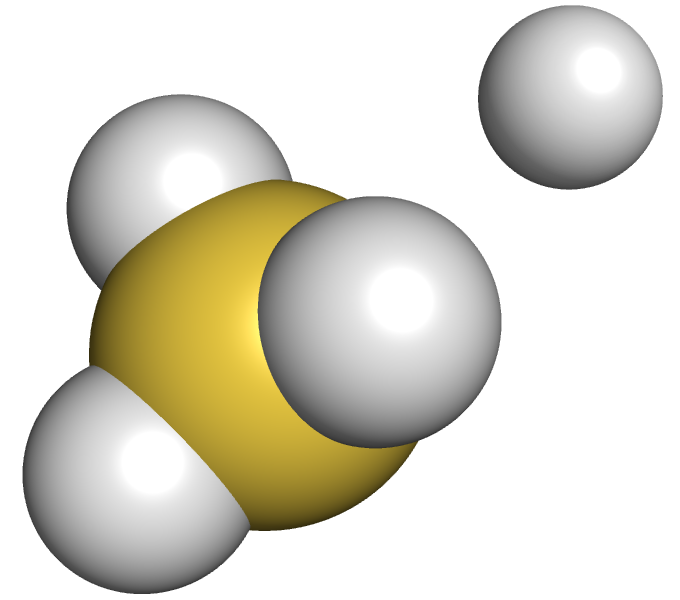
\includegraphics[width=\textwidth]{silane_narayanan_unstable}
    \subcaption{narayanan: instabil}
  \end{subfigure}
  \hfill
  \begin{subfigure}[t]{5cm}
    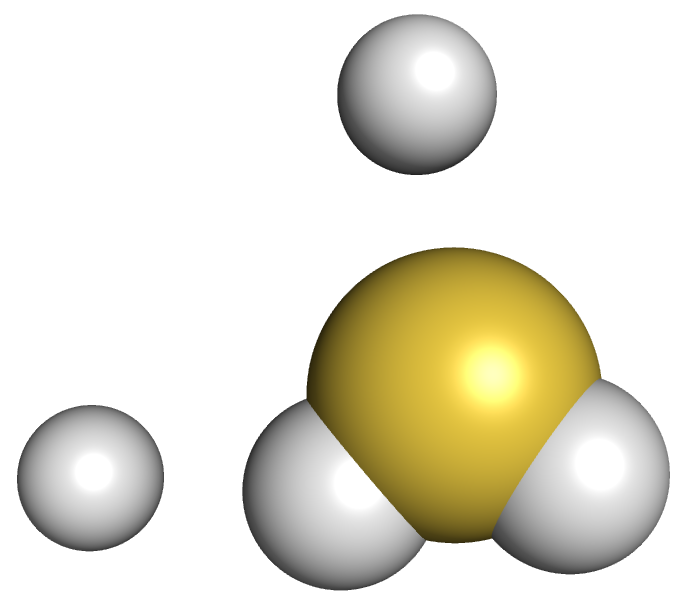
\includegraphics[width=\textwidth]{silane_liu_unstable}
    \subcaption{liu-ettringite: instabil}
  \end{subfigure}

  \caption{Stabilitätsuntersuchungen von Silan (\ce{SiH4}) bei \SI{600}{\kelvin}}
  \label{fig:silanestability}

\end{figure}

\section{Reaktion der Precursormoleküle}

Reaktionen von einzelnen Precursormolekülen wurden stichprobenartig in verschiedenen Orientierungen, Energien und Temperaturen vorgenommen, um einen Überblick über die Verlässlichkeit der Reaktionsmechanismen zu bekommen (Abbildung~\ref{fig:precursorreactions}).
Einige Parametrisierungen zeigen vielversprechende Teilreaktionen, die korrekte Doppelbindungen und Bildung von Wasserstoffmolekülen beinhalten (Abbildung~\ref{fig:newsomereaction}).
Zusätzlich wurden durchmischte Precursorgase mit \num{6000} Atomen bei unterschiedlichen Dichten über eine außerordentlich lange Simulationszeiten von \SI{0.5}{\nano\second} mit dem Ziel eventueller Reaktionen simuliert, was jedoch mit keiner der Parametrisierungen zur Bildung physikalisch korrekter Strukturen führte (Abbildung~\ref{fig:precursorclusters}).
Vor allem bei größeren Simulationsräumen bilden sich aber Cluster aus Precursormolekülen, die von attraktiven Termen in den Kraftfeldern erzwungen werden, aber nicht durch chemische Wechselwirkungen zu erklären sind (Abbildung~\ref{fig:precursorclusters}).

Für die Reaktion von Silan mit Wasser wurden beide Moleküle außerhalb der Cutoff-Reich\-weite der ReaxFF-Potentiale (in der Regel \SI{6}{\angstrom}) mit zufälligen Orientierungen platziert und zusätzlich zu einer geringen Anfangsgeschwindigkeit zueinander beschleunigt.
Die relativen kinetischen Energien decken mit \SI{0.1}{\electronvolt} bis \SI{10}{\electronvolt}  einen breiten Bereich ab.

Die meisten Parametrisierungen zeigen keine Änderung des Bindungszustandes der Moleküle, allerdings treten bei \pot{zhang}, \pot{newsome} und \pot{kulkarni} Reaktionen auf.
Einige der \pot{zhang}-Simulationen zeigen eine Überzahl an stabilen Bindungen (Abbildung~\ref{fig:zhangreaction}), bei denen die \ce{O-O}-Bindungen gelegentlich gelöst werden, doch verringert sich die Wahrscheinlichkeit stabiler Überkoordinationen mit höheren Teilchenenergien und Temperaturen.
Die beiden anderen Potentiale zeigen meist die korrekte Zahl an Bindungen für das Silizium-Atom, doch bildet sich häufig atomarer Sauer- und Wasserstoff, der allerdings bei Kontakt mit einem anderen Atom Bindungen aufbauen müsste.
Dieses Verhalten konnte allerdings bisher nicht simuliert werden.

Bei der gleichzeitigen Reaktion vieler Precursor-Moleküle zeigen sich gravierendere Unterschiede (Abbildung~\ref{fig:precursorclusters}).
Kulkarni-Simulationen bilden etwa Sauerstoff-Cluster sowie Bindungen zwischen den Wasserstoff-Atomen verschiedener Silan-Moleküle.
Einzig der \pot{zhang}-Parametersatz stellt teilweise korrekte Bindungen dar, was vermutlich durch seine Anwendung zur Beschreibung der Reaktionen zwischen großen Moleküle verursacht wird.
Es zeigen sich jedoch auch hier Überkoordinationen, wie sie bereits in Abbildung~\ref{fig:precursorreactions} beobachtet werden konnten.

\begin{figure}[p]

  \captionsetup[subfigure]{singlelinecheck=false}
  \def\subfigwidth{0.32\textwidth}
  \begin{subfigure}[t]{3cm}
    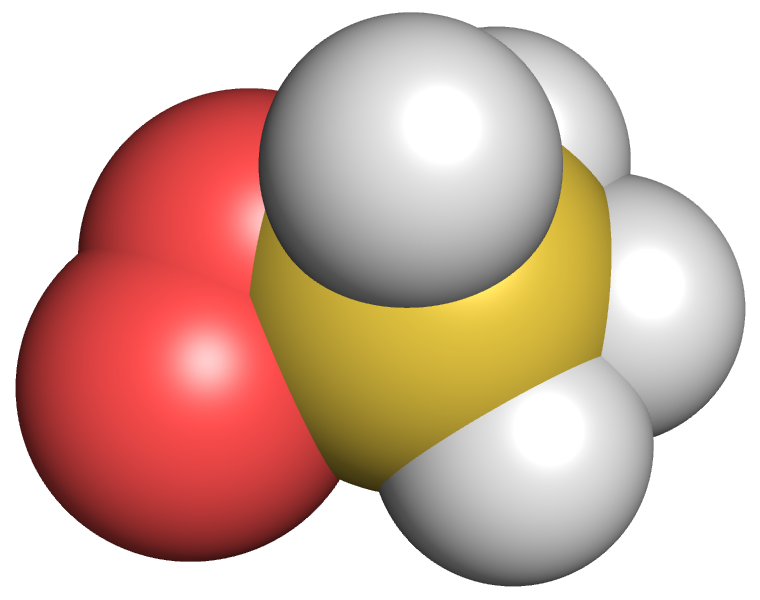
\includegraphics[width=\textwidth]{silane_reaction_zhang}
    \subcaption{\pot{zhang}: Überzahl an Bindungen}
    \label{fig:zhangreaction}
  \end{subfigure}
  \hfill
  \begin{subfigure}[t]{5cm}
    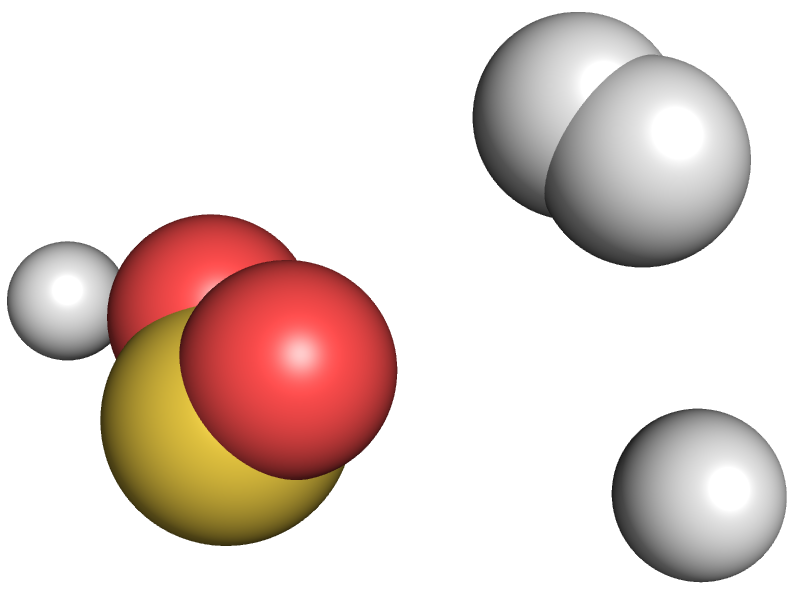
\includegraphics[width=\textwidth]{silane_reaction_newsome}
    \subcaption{\pot{newsome}: korrekte Stöchiometrie}
    \label{fig:newsomereaction}
  \end{subfigure}
  \hfill
  \begin{subfigure}[t]{4.5cm}
    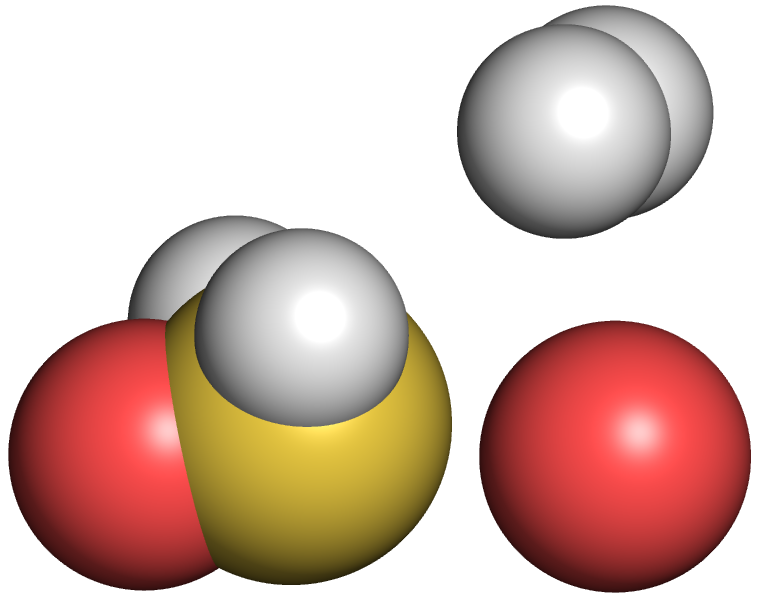
\includegraphics[width=\textwidth]{silane_reaction_kulkarni}
    \subcaption{\pot{kulkarni}: Korrekte \ce{Si}-Bindungen, aber \ce{O}-Atom}
    \label{fig:kulkarnireaction}
  \end{subfigure}

  \caption{ReaxFF-Simulationen der Reaktion von \ce{SiH4} mit \ce{O2}}
  \label{fig:precursorreactions}

\end{figure}

\begin{figure}[p]

  \captionsetup[subfigure]{singlelinecheck=false}
  \begin{subfigure}[t]{4cm}
    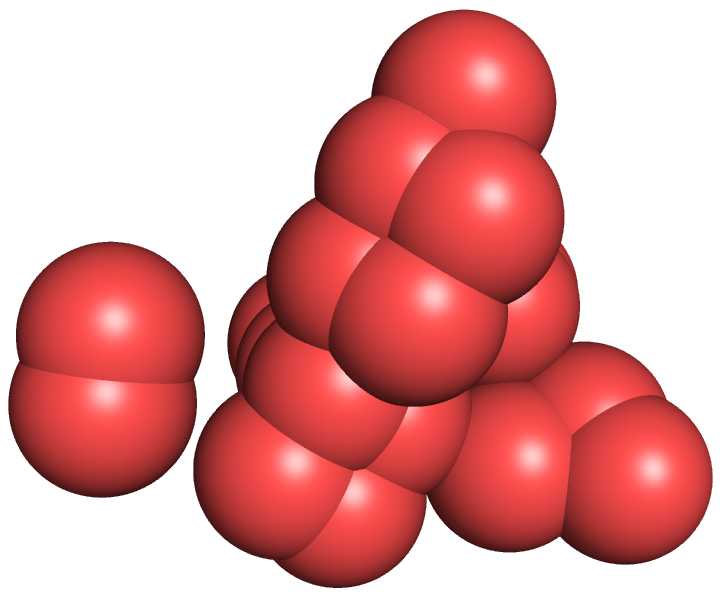
\includegraphics[width=\textwidth]{oxygen_cluster}
    \subcaption{\pot{kulkarni}: \ce{O2}-Cluster}
  \end{subfigure}
  \hfill
  \begin{subfigure}[t]{5.5cm}
    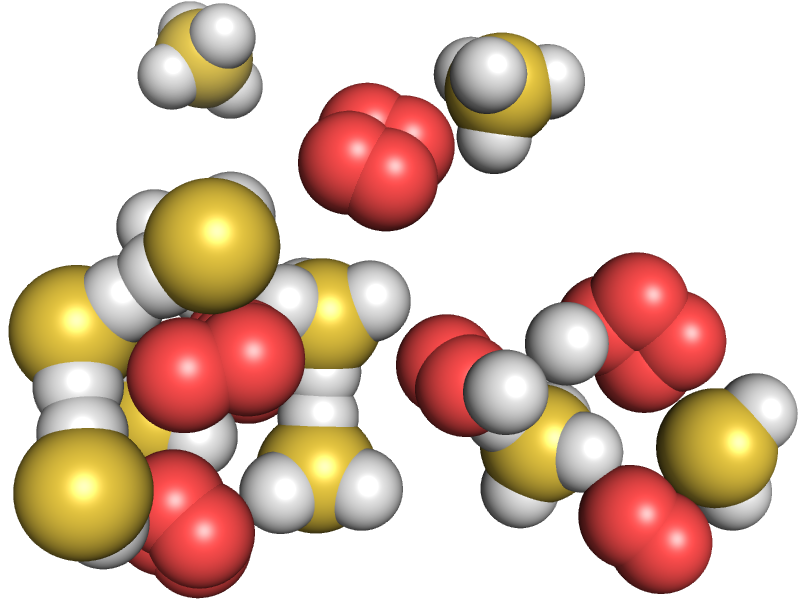
\includegraphics[width=\textwidth]{kulkarni_precursor_cluster}
    \subcaption{\pot{kulkarni}: Precursor-Cluster}
  \end{subfigure}
  \hfill
  \begin{subfigure}[t]{4.5cm}
    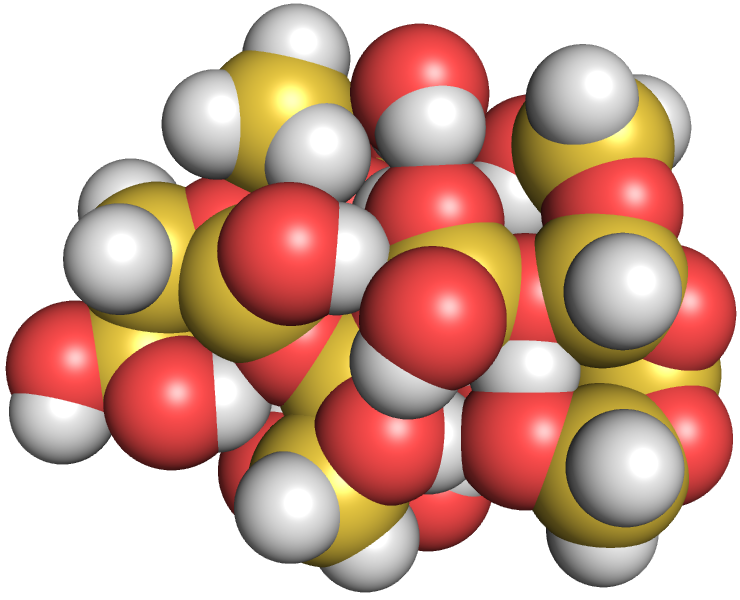
\includegraphics[width=\textwidth]{zhang_precursor_cluster}
    \subcaption{\pot{zhang}: Reaktionen}
  \end{subfigure}

  \caption[\ce{SiH4} mit \ce{O2}: Clusterbildung und partielle Reaktionen]{Simulation von Clusterbildung und partiellen Reaktionen von Precursormolekülen bei 500K}
  \label{fig:precursorclusters}

\end{figure}
